\documentclass[10pt,a4paper]{article}
\usepackage[latin1]{inputenc}
\usepackage{amsmath}
\usepackage{amsfonts}
\usepackage{amssymb}
\usepackage{graphicx}
\usepackage{soul}
\usepackage[left=2cm,right=2cm,top=2cm,bottom=2cm]{geometry}
\author{Akshat Mahajan}
\title{Physics 180Q - Lab Report 1}
\begin{document}
\maketitle
\textsl{The responsivity of our photodiode is 0.3 A/W. Inverting this ratio, we obtain 3.334 W/A. This lab was performed in conjunction with Hanwen Qin.}
\section*{Part 1: Aligning a Laser Beam Through Two Points in Space}
We directed a beam level with the optical table through two fixed apertures on the table, using two mirrors. We followed a three step process, namely a) centering the light from the mirror closest to the laser on the aperture closest to the laser, b) centering the beam from the mirror furthest from the laser on the aperture furthest from the laser, upsetting the centering from the last step c) repeat until convergence.
\begin{enumerate}
\item Why is convergence of the beams guaranteed?

\textbf{Answer}: \ul{Convergence of the beams occurs because the corrections induced by this procedure became smaller and smaller at every iteration}. To clarify: there is only one path that passes through both apertures. By aligning the upstream mirror with the upstream aperture first, we first guarantee that the beam is able to pass through the first aperture. The path of the beam from the upstream to the downstream mirror is then fixed; if it is the right path, then all we're doing is correcting the beam's path from the second mirror to center on the second aperture. If this cannot be done, we can conclude the overall path is not correct, and can go back to varying the upstream mirror to center on the upstream mirror while ensuring at least part of the beam is incident on the apertures. Each time we do this, the corrections grow smaller and smaller because we reduce the number of possible orientations of the mirrors each time. This is why this method guarantees convergence.
\item What happens if you invert the process [of aligning a beam through two points] i.e. if you use the downstream (furthest) mirror to align the beam to the upstream (closest) iris?

\textbf{Answer}:  As before, we emphasise there is only one correct path through the apertures. The issue with the stated approach is that \ul{the path of the beam from the upstream mirror to the downstream mirror is no longer fixed at each subsequent adjustment}. Varying the upstream mirror to align the beam with the downstream iris requires that the path of the beam from the upstream onwards should change with no guarantee that it is the wrong path with the beam not necessarily incident on the apertures (whereas we only proceeded along this step with the guarantee that it wasn't right) - so we might have stumbled on the right path, but might move away from it until we find it again. It is a very inefficient method of finding the path, and convergence is \textit{not} guaranteed.  
\end{enumerate}

\section*{Part 2: Using a Photodiode and Oscilloscope}
We measured the  power of the laser using a photodiode and an oscilloscope with a variable impedance terminator. We had to ensure that the scope impedance was set to 1 M$\Omega$ before anything else could be done. For this portion, the lights were on - but we measured the background correction and were able to arrive at a background-corrected value for the power. Our somewhat low value of 11.2 V at 50 k$\Omega$ was obtained after the laser accidentally dropped to the floor and the power settings button was found to be slightly misaligned. 
\begin{enumerate}
\item Calculate the power of the laser for each impedance [as recorded on the variable impedance terminator]. Explain your results. 

\textbf{Answer}: See Table 1 below. To obtain power, we multiplied 3.334 W/A (inverted responsivity) with the current (voltage divided by impedance).

We see that our results peak at 500 $\Omega$, exhibiting trends away from this value as impedance is increased or decreased. While we currently have no proven explanation for this odd trend, we do think there may be nonlinear trends involved in the oscilloscope construction or that our value for the responsivity may be prone to error. 
\begin{table}[h]
\centering
\begin{tabular}{|ccccc|}
\hline 
Impedance & Measured Voltage & Background Correction & Corrected Voltage & Power \\
\hline 
50 k$\Omega$ & 11.2 $\pm$ 0 V & 56 $\pm$ 3 mV & 11.1944 V & 0.7 mW \\ 
\hline 
10 k$\Omega$ & 2.67 $\pm$ 0.2 V & 23 $\pm$ 1 mV & 2.667 V & 0.8 mW \\ 
\hline 
5 k$\Omega$ & 1.38 V & 15.0 $\pm$ 5 mV & 1.3775 V & 0.9 mW \\ 
\hline 
1 k$\Omega$ & 370 $\pm$ 3 mV & 19 $\pm$ 5 mV & 351 mV & 1.1 mW \\ 
\hline 
500 $\Omega$ & 197 $\pm$ 1 mV & 17 $\pm$ 3 mV & 180 mV & 1.2 mW \\ 
\hline 
100 $\Omega$ & 49 $\pm$ 15 mV & 17 $\pm$ 3 mV & 32 mV & 1.0 mW \\ 
\hline 
50 $\Omega$ & 29 $\pm$ 2 mV & 15 $\pm$ 4 mV & 14 mV & 0.9 mW \\ 
\hline 
\multicolumn{5}{c}{Average Power: 0.94 mV}\\
\hline
\end{tabular}
\caption{Table relevant to Part 2, Question 1.}
\end{table}

\item Also, explain why you had to set the scope impedance to 1M$\Omega$ for the variable impedance terminator to work. 

\textbf{Answer}: The input impedance of our oscilloscope (a TDS2014 Tektronix oscilloscope) is by default 1 M$\Omega$ in parallel with 20 pF (according to the user manual). This is a (rough) sketch of how an oscilloscope works:
\begin{figure}[h]
\centering
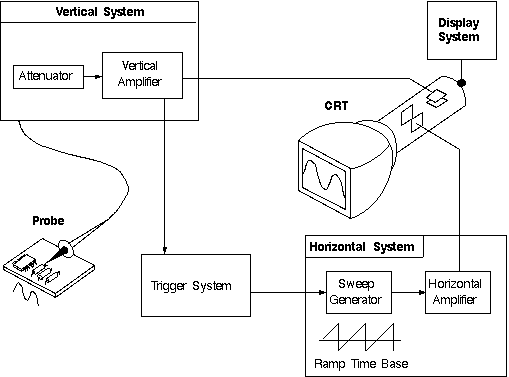
\includegraphics[scale = 0.8]{oscillosco6_06.png} 
\end{figure} 
They key insight here is that an oscilloscope makes use of an attenuator to reduce the signals below some key threshold, in order to avoid burning out the device. This attenuator is characterised by an impedance, here designed to be 1 M$\Omega$. By setting the scope impedance to zero, we are ensuring that the system receives signals only in the range that it can, itself, handle.
\item What class of laser is this?

\textbf{Answer}: This is a \textbf{Class 2} laser (output $<$ 1 mW). Our laser is capable of going up to a Class 3b laser, but the power settings were fixed otherwise.
\item Using the same basic procedure, measure the power exiting the first and last apertures [from the previous part]. Calculate the fraction of light you coupled through each aperture and the total coupling efficiency through both.

\textbf{Answer}: See Tables 2 and 3 below. Values that fall within the background correction range should not be given credence.
\begin{table}[h]
\centering
\begin{tabular}{|cccccp{2cm}|}
\hline 
Impedance & Measured Voltage & Background Correction & Corrected Voltage & Power & Fraction\footnotemark \\
\hline 
50 k$\Omega$ & 10 $\pm$ 0 V & 56 $\pm$ 3 mV & 9.9440 V & 0.6 mW & 85.7\% \\ 
\hline 
10 k$\Omega$ & 2.13 $\pm$ 0.01 V & 23 $\pm$ 1 mV & 1.90 V & 0.7 mW & 87.5\% \\ 
\hline 
5 k$\Omega$ & 1.02 $\pm$ 0.01 V & 15.0 $\pm$ 5 mV & 0.87 V & 0.6 mW & 66.7\% \\ 
\hline 
1 k$\Omega$ & 257 $\pm$ 3 mV & 19 $\pm$ 5 mV & 238 mV & 0.7 mW & 63.6\% \\ 
\hline 
500 $\Omega$ & 174 $\pm$ 2 mV & 17 $\pm$ 3 mV & 157 mV & 1.0 mW & 83.33\% \\ 
\hline 
100 $\Omega$ & 38 $\pm$ 15 mV & 17 $\pm$ 3 mV & 21 mV & 0.7 mW & 70\%\\ 
\hline 
50 $\Omega$ & 29 $\pm$ 2 mV & 15 $\pm$ 4 mV & 14 mV & 0.9 mW & 100\%\\ 
\hline 
\end{tabular}
\caption{Table relevant to Part 2, Question 4. (Power Through First Aperture)}
\end{table}
\footnotetext{Of original light; see Table 1 for reference values.}
\begin{table}[h]
\centering
\begin{tabular}{|p{2cm}p{2cm}p{2cm}p{2cm}p{2cm}p{2cm}p{2cm}|}
\hline 
Impedance & Measured Voltage & Background Correction & Corrected Voltage & Power & Fraction\footnotemark & Coupling Efficiency\footnotemark \\
\hline 
50 k$\Omega$ & 7.70 $\pm$ 0.2 V & 56 $\pm$ 3 mV & 7.644 V & 0.53 mW & 75.67\% & 88.3\% \\ 
\hline 
10 k$\Omega$ & 2.13 $\pm$ 0.01 V & 23 $\pm$ 1 mV & 1.617 V & 0.53 mW & 66.23\% & 75.7\% \\ 
\hline 
5 k$\Omega$ & 802 $\pm$ 1 mV & 15.0 $\pm$ 5 mV & 787 mV & 0.52 mW & 57.80\% & 86.67\% \\ 
\hline 
1 k$\Omega$ & 208 $\pm$ 2 mV & 19 $\pm$ 5 mV & 189 mV & 0.63 mW & 57.24\% & 90\% \\ 
\hline 
500 $\Omega$ & 150 $\pm$ 3 mV & 17 $\pm$ 3 mV & 133 mV & 0.87 mW & 72.47\% & 87\% \\ 
\hline 
100 $\Omega$ & 33.3 $\pm$ 2 mV & 17 $\pm$ 3 mV & 16.5 mV & 0.61 mW & 60.9\% & 87\%\\ 
\hline 
50 $\Omega$ & 23 $\pm$ 3 mV & 15 $\pm$ 4 mV & 8 mV & 0.53 mW & 58.88\% & 58.88\%\\ 
\hline 
\end{tabular}
\caption{Table relevant to Part 2, Question 4. (Power Through Second Aperture)}
\end{table}
\footnotetext{Of original light; see Table 1 for reference values.}
\footnotetext{Fraction of light through first aperture; see Table 2 for reference values.}
\end{enumerate}

\section*{Part 3: Aligning a Lens to a Beam}
We performed experiments on the influence of a lens on the power of a laser beam. We placed the lens in the middle of the fixed apertures. 
\begin{enumerate}
\item Explain why [taking the forward non-deviation measurement] verifies that light is going through the center of the lens.

\textbf{Answer}: The forward non-deviation measurement takes advantage of the fact that light that does not pass through the optical center is bent towards the focus. Keeping the lens at level height, then, we know then that any light beam that is not passing through the center of the lens will be bent away from the original spot (i.e. through the aperture). Logically, the contrapositive - light that passes through the second aperture passes through the center of the lens - must be true.
\item Now measure the fraction of light getting through the last aperture [after rotating the lens so that the back reflection overlaps with the incoming beam in the horizontal plane]. How much did the lens improve your coupling efficiency?

\textbf{Answer}: See Table 4.

\begin{table}[h]
\centering
\begin{tabular}{|cccccp{2cm}|}
\hline 
Impedance & Measured Voltage & Background Correction & Corrected Voltage & Power & Improvement\footnotemark \\
\hline 
50 k$\Omega$ & 9.62 $\pm$ 0.01 V & 56 $\pm$ 3 mV & 9.9440 V & 0.63 mW & 90\% \\ 
\hline 
10 k$\Omega$ & 2.02 $\pm$ 0.01 V & 23 $\pm$ 1 mV & 1.90 V & 0.66 mW & 82.5\% \\ 
\hline 
5 k$\Omega$ & 1.02 $\pm$ 0 V & 15.0 $\pm$ 5 mV & 0.87 V & 0.67 mW & 60.3\% \\ 
\hline 
1 k$\Omega$ & 253 $\pm$ 4 mV & 19 $\pm$ 5 mV & 238 mV & 0.7 mW & 78.0\% \\ 
\hline 
500 $\Omega$ & 178 $\pm$ 3 mV & 17 $\pm$ 3 mV & 157 mV & 1.07 mW & 89.16\% \\ 
\hline 
100 $\Omega$ & 39 $\pm$ 2 mV & 17 $\pm$ 3 mV & 21 mV & 0.73 mW & 73\%\\ 
\hline 
50 $\Omega$ & 27 $\pm$ 3 mV & 15 $\pm$ 4 mV & 14 mV & 0.8 mW & 88.88\%\\ 
\hline 
\end{tabular}
\caption{Table relevant to Part 3, Question 2.}
\end{table}
\footnotetext{Fraction of light through second aperture. This is not the total coupling efficiency. Compare with Column 6, Table 3.}
\item Now, purposely rotate the lens a little so that you can use an additional mirror to redirect the back reflected light onto the photodiode. Measure the power in the back-reflected beam. Calculate the fraction of light back reflected by the lens.

\textbf{Answer}: See Table 5. We measured the back reflection with the lights off, so there is now no background correction. \textbf{An asterisk (*)} denotes that the signal falls within the range of background noise at that level, and should not be trusted as a valid measure.
\begin{table}[h]
\centering
\begin{tabular}{|p{2cm}p{2cm}p{2cm}p{2cm}|}
\hline 
Impedance & Measured Voltage & Power & Fraction\footnotemark \\
\hline 
50 k$\Omega$ & 134 $\pm$ 3 mV & 8 $\mu$V & 1.34 \% \\ 
\hline 
10 k$\Omega$ & 33 $\pm$ 1 mV & 11 $\mu$V & 1.73 \% \\ 
\hline 
5 k$\Omega$ & 23 $\pm$ 3 mV & 76 $\mu$V & 2.64\% \\ 
\hline 
1 k$\Omega$ & 15* $\pm$ 5 mV & 50 $\mu$V & 6.3\% \\ 
\hline 
500 $\Omega$ & 16.6* $\pm$ 0 mV & 110 $\mu$V & 10.5\% \\ 
\hline 
100 $\Omega$ & 16.6* $\pm$ 0 mV & 0.5 mW & 79\% \\ 
\hline 
50 $\Omega$ & 16.6* $\pm$ 0 mV & 1.1 mW & 118\%\\ 
\hline 
\end{tabular}
\caption{Table relevant to Part 3, Question 3.}
\end{table}
\footnotetext{Fraction of light through first aperture i.e. light incident on lens.}
\item The lens is made from fused silica and is uncoated. Does this back-reflected fraction make sense with what you would expect?

\textbf{Answer}: Fresnel's equations predict about \textbf{3\%} backreflection. The values measured (excluding those that are virtually indistinguishable from background noise at that level) are reasonably close to that value. The Fresnel equations assume perfect transmission, which need not be the case - misalignment, lens aberrations, and other things could have played a role here (although care was taken to minimise their influence).
\end{enumerate}

\section*{Part 4: Aligning a beam splitter}
We verified the effects of a beam splitter on the laser beam. At this stage, Professor Hudson removed both apertures, so we retook the power measurements emitting immediately out of the laser emitter.
\begin{enumerate}
\item Verify that the beam is a 50:50 beam splitter.

\textbf{Answer}: See Table 6. For this scenario, we need only consider the voltages, as power is simply a multiple of the voltage. Given the small nature of the background corrections (exhibited in previous tables) compared to the values, we will not be including them in this table. A proper calculation may be derived by incorporating them explicitly everywhere; with the exception of those marked with an asterisk, however, the correction is anticipated to be small.\\
\\
An asterisk (*) indicates that the ratios do not appear to add up close to 100. Again, these signals are relatively close to the background level (see other tables) that it is possible that misreadings have occurred. We see generally, however, that the beam appears to be anisotropic, and that the beam is \textsl{not} a 50:50 beam splitter.
\begin{table}[h]
\centering
\begin{tabular}{|p{2cm}p{2cm}p{2cm}p{2cm}p{2cm}|}
\hline
Impedance & Voltage Prior & Voltage Forward & Voltage Sideways & Proportion\\
\hline
50 k$\Omega$ & 11.2 V & 5 $\pm$ 0.01 V & 7.39 V & 45:55\\
\hline
10 k$\Omega$ & 2.78 V & 1.04 $\pm$ 0.01 V & 1.59 V & 40:60\\
\hline
5 k$\Omega$ & 1.40 V & 535 $\pm$ 5 mV & 799 mV & 40:60\\
\hline
5 k$\Omega$ & 1.40 V & 535 $\pm$ 5 mV & 799 mV & 40:60\\
\hline
1 k$\Omega$ & 375 $\pm$ 5 mV & 180 $\pm$ 2 mV & 205 $\pm$ 1 mV & 48:52\\
\hline
500 $\Omega$ & 199 $\pm$ 1 mV & 102 $\pm$ 10 mV & 140 $\pm$ 5 mV & 54:70(*)\\
\hline
100 $\Omega$ & 48 $\pm$ 5 mV & 28 $\pm$ 4 mV & 30 $\pm$ 4 mV & 58:62(*)\\
\hline
50 $\Omega$ & 29 $\pm$ 3 mV & 21 $\pm$ 1 mV & 22.8 $\pm$ 3 mV & 72:73(*)\\
\hline
\end{tabular}
\caption{Table relevant to Part 4, Question 1.}
\end{table}
\end{enumerate}
\end{document}